% !TEX root = doc.tex
% Copyright (c) 2016 The ALF project.
% This is a part of the ALF project documentation.
% The ALF project documentation by the ALF contributors is licensed
% under a Creative Commons Attribution-ShareAlike 4.0 International License.
% For the licensing details of the documentation see license.CCBYSA.

%------------------------------------------------------------
%\section{Monte Carlo sampling}\label{sec:sampling}
%-------------------------------------------------

Error estimates in Monte Carlo simulations are based on the central limit theorem~\cite{Negele} and can be a delicate matter, especially as it requires independent measurements and a finite variance. In this section we give examples of the care that must be taken to satisfy these requirements when using a Monte Carlo code. This is part of the common lore of the field and we cover them briefly in this text.
For a deeper understanding of the inherent issues of Markov-chain Monte Carlo methods we refer the reader to the pedagogical introduction in chapter 1.3.5 of Krauth~\cite{Krauth2006}, the overview article of Sokal~\cite{Sokal89},  the more specialized literature by Geyer~\cite{Geyer1992} and chapter 6.3 of Neal~\cite{neal1993}.

In general, one distinguishes local from global updates. As the name suggest, the local update corresponds to a small change of the configuration, e.g., a single spin flip of one of the $L_{\mathrm{Trotter}}(M_I+M_V)$ field entries (see Sec.~\ref{sec:updating}), whereas a global update changes a significant part of the configuration. The default update scheme of the ALF implementation are local updates, such that there is a minimum number of moves required for generating an independent configuration. The associated time scale is called  the autocorrelation time, $T_\mathrm{auto}$, and is generically dependent upon the choice of the observables. 

We call a \textit{sweep} a sequential propagation from $\tau = 0$ to $\tau = L_{\text{ Trotter}}$ and back, such that each field is visited twice in each sweep. A single sweep will generically not suffice to produce an independent configuration.
In fact, the autocorrelation time $T_\mathrm{auto}$ characterizes the required time scale to generate independent values of $\langle\langle\hat{O}\rangle\rangle_C$ for the observable $O$. This has several consequences for the Monte Carlo simulation:
\begin{itemize}
	\item First of all, we start from a randomly chosen field configuration, such that one has to invest a time of \emph{at least} one $T_\mathrm{auto}$, but typically many more, in order to generate relevant, equilibrated configurations before reliable measurements are possible. This phase of the simulation is known as the warm-up or burn-in phase. In order to keep the code as flexible as possible (as different simulations might have different autocorrelation times), measurements are taken from the very beginning and, in the analysis phase, the parameter \path{n_skip} controls the number of initial bins that are ignored.
	\item Second, our implementation averages over bins with \texttt{NSWEEPS} measurements before storing the results on disk. The  error analysis requires statistically  independent bins in order to generate reliable confidence estimates. If the bins are too small (averaged over a period shorter then $T_\mathrm{auto}$), then the error bars are typically underestimated. Most of the time, however, the autocorrelation time is unknown before the simulation is started and, sometimes, single runs long enough to generate appropriately sized bins are not feasible. For this reason, we provide a rebinning facility controlled by the parameter \path{N_rebin} that specifies the number of bins recombined into each new bin during the error analysis. One can test the suitability of a given bin size by verifying whether an increase in size changes the error estimate (For an explicit example, see Sec.~\ref{sec:autocorr} and the appendix of Ref.~\cite{Assaad02}).
	\item The \path{N_rebin} variable can be used to control a further issue. The distribution of the Monte Carlo estimates $\langle\langle\hat{O}\rangle\rangle_C$ is unknown, while a result in the form $(\mathrm{mean}\pm \mathrm{error})$ assumes a Gaussian distribution. Every distribution with a finite variance turns into a Gaussian one once it is folded often enough (central limit theorem). Due to the internal averaging (folding) within one bin, many observables are already quite Gaussian. Otherwise one can increase \path{N_rebin} further, even if the bins are already independent~\cite{Bercx17}.
	\item The last issue we mention concerns time-displaced correlation functions. Even if the configurations are independent, the fields within the configuration are still correlated. Hence, the data for $S_{\alpha,\beta}(\vec{k},\tau)$ (see Sec.~\ref{sec:obs}; Eq.~\eqref{eqn:s}) and $S_{\alpha,\beta}(\vec{k},\tau+\Delta\tau)$ are also correlated. Setting the switch \path{N_Cov = 1} triggers the calculation of the covariance matrix in addition to the usual error analysis. The covariance is defined by
	\begin{align}
		COV_{\tau\tau'}=\frac{1}{N_{\text{Bin}}}\left\langle
		\left( S_{\alpha,\beta}(\vec{k},\tau) - \big\langle S_{\alpha,\beta}(\vec{k},\tau)\big\rangle \right)
		\left(S_{\alpha,\beta}(\vec{k},\tau')-\big\langle S_{\alpha,\beta}(\vec{k},\tau')\big\rangle \right)  \right\rangle\,.
	\end{align}
An example where this information is necessary is the  calculation of mass gaps extracted by fitting the  tail  of the time-displaced correlation function.  Omitting  the covariance matrix will  underestimate the  error.
\end{itemize}


%
%--------------------------------------------------------------
\subsection{The Jackknife resampling method}\label{sec:jack}
%--------------------------------------------------------------
%
For each observable $\hat{A}, \hat{B},\hat{C} \cdots$ the Monte Carlo program computes a data set of $N_{\text{Bin}}$ (ideally) independent values where for each observable the measurements belong to the same  statistical distribution.  In the general case, we would like to evaluate a function of expectation values, $f(\langle \hat{A} \rangle, \langle \hat{B} \rangle, \langle \hat{C} \rangle  \cdots)$ --
see for example the expression (\ref{eqn:obs_rw}) for the observable including reweighting --
and are interested in the statistical estimates of its mean value  and the standard error of the mean.
A numerical method for the statistical analysis of a given function $f$ which properly handles error propagation and correlations among the observables is the Jackknife method, which is, like the related Bootstrap method, a resampling scheme \cite{efron1981}.
Here we briefly review the \textit{delete-1 Jackknife} scheme, which consists in generating $N_{\text{bin}}$ new data sets of size $N_{\text{bin}}-1$ by consecutively removing one data value from the original set. By $A_{(i)}$ we denote the arithmetic mean for the observable $\hat{A}$, without the $i$-th data value $A_{i}$, namely
\begin{equation}
A_{(i)} \equiv \frac{1}{N_{\text{Bin}}-1} \sum\limits_{k=1,\,k\neq i}^{N_{\text{Bin}}} A_{k}\;.
\end{equation}
As the corresponding quantity for  the function $f(\langle \hat{A} \rangle, \langle \hat{B} \rangle, \langle \hat{C} \rangle  \cdots)$, we define 
\begin{equation}
f_{(i)}(\langle \hat{A} \rangle, \langle \hat{B} \rangle, \langle \hat{C} \rangle  \cdots) \equiv
f( A_{(i)}, B_{(i)},C_{(i)}\cdots)\;.
\end{equation}
Following the convention in the literature, we will denote the final Jackknife estimate of the mean by $f_{(\cdot)}$ and its standard error by $\Delta f$. The Jackknife mean is  given by
\begin{equation}
\label{eqn:jack_mean}
f_{(\cdot)}(\langle \hat{A} \rangle, \langle \hat{B} \rangle, \langle \hat{C} \rangle  \cdots) =
\frac{1}{N_{\text{Bin}}}\sum\limits_{i=1}^{N_{\text{Bin}}} f_{(i)}(\langle \hat{A} \rangle, \langle \hat{B} \rangle, \langle \hat{C} \rangle  \cdots)\;,
\end{equation}
and the standard error, including bias correction, is given by
\begin{equation}
\label{eqn:jack_error}
(\Delta f)^{2} = 
\frac{N_{\text{Bin}}-1}{N_{\text{Bin}}} \sum\limits_{i=1}^{N_{\text{Bin}}}
\left[f_{(i)}(\langle \hat{A} \rangle, \langle \hat{B} \rangle, \langle \hat{C} \rangle  \cdots)
- f_{(\cdot)}(\langle \hat{A} \rangle, \langle \hat{B} \rangle, \langle \hat{C} \rangle  \cdots)\right]^{2}\;.
\end{equation}
For $f=\langle\hat A\rangle$, the equations (\ref{eqn:jack_mean}) and (\ref{eqn:jack_error}) reduce to the plain sample average and the standard, bias-corrected, estimate of the error.

%
%--------------------------------------------------------------------------
\subsection{An explicit example of error estimation}\label{sec:autocorr}
%---------------------------------------------------------------------------
%
In the following we use one of our examples, the Hubbard model on a square lattice in the $M_z$ HS decoupling (see Sec.~\ref{sec:hubbard}), to show explicitly how to estimate errors.  We show as well that the  autocorrelation time is dependent on the  choice of observable.  In fact, different observables within the same run can have different autocorrelation times and, of course, this time scale depends on the  parameter choice.  Hence, the user has to check  autocorrelations of individual observables for each simulation!  Typical regions of the phase diagram that require special attention are critical points  where length scales diverge.  

In order to determine the autocorrelation time, we calculate the correlation function
\begin{equation}
\label{eqn:autocorrel}
	S_{\hat{O}}(t_{\textrm{Auto}})=\sum_{i=1}^{N_{\textrm{Bin}}-t_{\textrm{Auto}}}\frac{\left(O_i-\left\langle \hat{O}\right\rangle \right)\left(O_{i+t_{\textrm{Auto}}}-\left\langle \hat{O}\right\rangle \right)}{\left(O_i-\left\langle \hat{O}\right\rangle \right)\left(O_{i}-\left\langle \hat{O}\right\rangle \right)}\, ,
\end{equation}
where $O_i$ refers to the Monte Carlo estimate of the observable $\hat{O}$ in the $i^{\text{th}}$ bin. This function typically shows an exponential decay and the decay rate defines the autocorrelation time.
%
\begin{figure}
	\begin{center}
		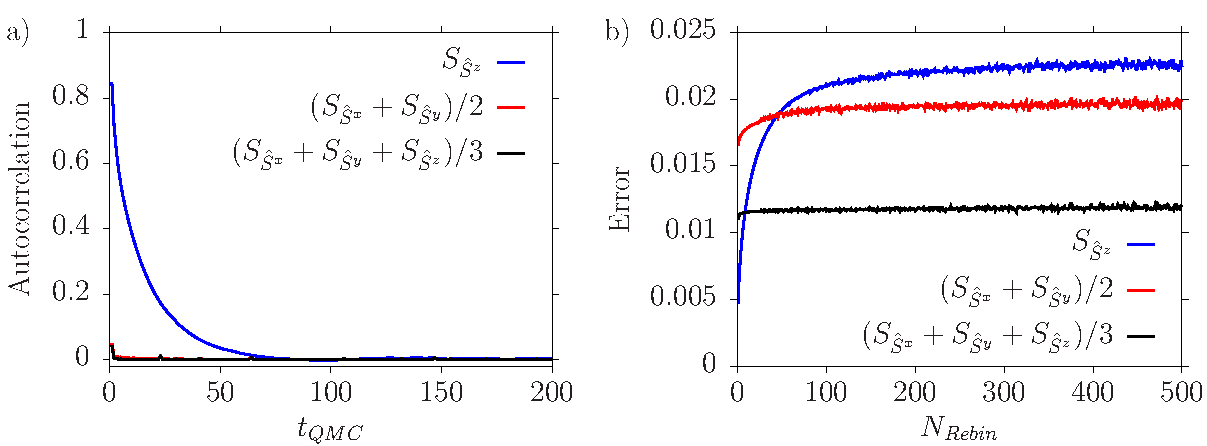
\includegraphics[width=.95\textwidth]{Figures/fig1.pdf}
		\caption{The autocorrelation function $S_{\hat{O}}(t_{\textrm{Auto}})$ (a) and the scaling of the error with effective bin size (b) of three equal-time, spin-spin correlation functions $\hat{O}$ of the Hubbard model in the $M_z$ decoupling (see Sec.~\ref{sec:hubbard}). Simulations were done on a $ 6 \times 6$ square lattice, with  $U/t=4$ and $\beta t = 6$. We used $\textrm{\texttt{N\_auto}}=500$ (see Sec.~\ref{sec:running}) and a total of approximately one million bins. The original bin contained only one sweep and we calculated around one million bins on a single core. The different  autocorrelation times for the $xy$-plane compared to the $z$-direction can be detected from the decay rate of the autocorrelation function (a) and from the point where saturation of the error sets in (b), which defines the required effective bin size for independent measurements. The improved estimator $(S_{\hat{S}^{x}} + S_{\hat{S}^{y}}+ S_{\hat{S}^{z}})/3$ appears to have the smallest autocorrelation time, as argued in the text.}
		\label{fig_autocorr}
	\end{center}
\end{figure}
%
Figure~\ref{fig_autocorr}(a) shows the autocorrelation functions $S_{\hat{O}}(t_{\textrm{Auto}})$ for three spin-spin-correlation functions [Eq.~(\ref{eqn:s})] at momentum $\vec{k}=(\pi,\pi)$ and at $\tau=0$: 

$\hat{O} = S_{\hat{S}^{z}}$ for the $z$ spin direction, 
$\hat{O} =(S_{\hat{S}^{x}} + S_{\hat{S}^{y}})/2$ for the $xy$ plane, and
$\hat{O} =(S_{\hat{S}^{x}} + S_{\hat{S}^{y}}+ S_{\hat{S}^{z}})/3$ for the total spin.
The Hubbard model has an SU(2) spin symmetry. However, we chose a HS field which couples to the $z$-component of the magnetization,  $M_z$,  such that each individual configuration breaks this symmetry. Of course, after Monte Carlo averaging one expects restoration of the symmetry. The model, on bipartite  lattices,  shows spontaneous spin-symmetry breaking at $T=0$ and in the thermodynamic limit.  At finite temperatures, and within the so-called renormalized classical regime,  quantum antiferromagnets have a length scale  that  diverges  exponentially  with decreasing temperatures \cite{Chakravarty88}.     
The parameter set chosen for Fig.~\ref{fig_autocorr}  is non-trivial in the sense that it places the Hubbard model in this renormalized classical regime where the correlation length is substantial.  Figure~\ref{fig_autocorr}  clearly shows a very short autocorrelation time for the $xy$-plane whereas we detect a considerably longer  autocorrelation time  for the $z$-direction.  This is a direct consequence of the \emph{long} magnetic length scale and the chosen decoupling.
The physical reason for the long autocorrelation time  corresponds to  the restoration of the SU(2) spin symmetry.    This insight can be used to define an improved, SU(2) symmetric estimator for the spin-spin correlation function, namely
$(S_{\hat{S}^{x}} + S_{\hat{S}^{y}} + S_{\hat{S}^{z}})/3$. 
Thereby, global spin rotations are no longer an issue and this improved estimator  shows the shortest autocorrelation time, as can be clearly seen in Fig.~\ref{fig_autocorr}(b). Other ways to tackle large autocorrelations are global updates and parallel tempering.

A simple method to obtain estimates of the mean and its standard error from the time series of Monte Carlo samples is provided by the aforementioned facility of rebinning. Also known in the literature as rebatching, it consists in aggregating a fixed number \path{N_rebin} of adjacent original bins into a new effective bin.
In addition to measuring the decay rate of the autocorrelation function (Eq.~\eqref{eqn:autocorrel}), a measure for the autocorrelation time  can be also obtained by the rebinning method. 
For a comparison to other methods of estimating the autocorrelation time we refer the reader to the literature \cite{Thompson2010, Geyer1992, neal1993}.
A reliable error analysis requires independent bins, otherwise the error is typically underestimated. This behavior is observed in Fig.~\ref{fig_autocorr} (b), where the effective bin size is systematically increased by rebinning. If the effective bin size is smaller than the autocorrelation time the error will be underestimated. When the effective bin size becomes  larger than the autocorrelation time, converging behavior sets in and the error estimate becomes reliable.


%------------------------------------------------------------
\subsection{Pseudocode description}\label{sec:pseudocode}
%------------------------------------------------------------

The Monte Carlo algorithm as implemented in ALF is summarized in Alg.~\ref{alg:1}. Key control variables include:
\begin{description}[leftmargin=!,align=right,noitemsep,labelwidth=\widthof{\bfseries Global\_moves},font=\texttt] % width: The longest label
	\item[Projector]     Uses (=true) the projective instead of finite-$T$ algorithm (see Sec.~\ref{sec:defT0})
	\item[$L_{\tau}$]    Measures (Ltau=1) time-displaced observables (see Sec.~\ref{sec:Observables.General})
	\item[Tempering]     Runs (=true) in parallel tempering mode (see Table~\ref{table:Updating_schemes})
	\item[Global\_moves] Carries out (=true) global moves in a single time slice (see Table~\ref{table:Updating_schemes}) 
	\item[Sequential]    Carries out (=true) sequential, single spin-flip updates (see Table~\ref{table:Updating_schemes})
	\item[Langevin]      Uses (=true) Langevin dynamics instead of sequential (see Table~\ref{table:Updating_schemes})
\end{description}
Per default, the finite-temperature algorithm is used, \texttt{Ltau=0}, and the updating used is \texttt{Sequential} (i.e., \texttt{Global\_moves}, \texttt{Tempering} and \texttt{Langevin} default values are all \texttt{.false.}).

%\begin{algorithm}[H]
\begin{breakablealgorithm}
	\caption{Basic structure of the QMC implementation in \texttt{Prog/main.f90}}
	\label{alg:1}
	\begin{algorithmic}[1]
		
		\LineComment{\textsc{Initialization}}
		\State{\textbf{call} Ham\_Set}\Comment{Set the Hamiltonian and the lattice}
		\State{\textbf{call} Fields\_Init}\Comment{Set the auxiliary fields}
		\State{\textbf{call} Nsigma\%in}\Comment{Read in an auxiliary-field configuration or generate it randomly}
		\For{$n=L_{\text{Trotter}}$ to $1$} \Comment{Fill the storage needed for the first actual MC sweep}
		\State{\textbf{call} Wrapul}\Comment{Compute propagation matrices and store them at stabilization points}
		\EndFor
		\vspace{1.5ex}
		
		\LineComment{\textsc{Monte Carlo run}}
		\For{$n_{\text{bc}}=1$ to $N_{\text{Bin}}$}\Comment{Loop over bins. The bin defines the unit of Monte Carlo time}
		
		\For{$n_{\text{sw}}=1$ to $N_{\text{Sweep}}$}\Comment{\parbox[t]{0.6\linewidth}{Loop over sweeps. Each sweep updates twice (upward and downward in imaginary time) the space-time lattice of auxiliary fields}}
		
		\If{Tempering}
		\State{\textbf{call} Exchange\_Step} \Comment{Perform exchange step in a parallel tempering run}
		\EndIf
		\If{Global\_moves}
		\State{\textbf{call} Global\_Updates} \Comment{Perform chosen global updates}
		\EndIf
		\If{Langevin}
		\State{\textbf{call} Langevin\_update} \Comment{\textsc{Update and measure} equal-time observables}
		\If{$L_{\tau} = 1$}
		\If{Projector}
		\State{\textbf{call} Tau\_p} \Comment{\textsc{Measure} time-displaced observables (projective code)}
		\Else
		\State{\textbf{call} Tau\_m} \Comment{\textsc{Measure} time-displaced observables (finite temperature)}
		\EndIf
		\EndIf
		\EndIf \textcolor{gray}{~\scriptsize (Langevin)}
		\vspace{1.5ex}
		
		\If{Sequential}
		\vspace{1.5ex}
		
		\FirstLineComment{\textsc{Upward sweep}}
		\For{$n_{\tau}=1$ to $L_{\text{Trotter}}$}
		\State{\textbf{call} Wrapgrup}\Comment{\parbox[t]{0.6\linewidth}{\textsc{Propagate} Green function from $n_{\tau}-1$ to $n_{\tau}$, and compute its new estimate at $n_{\tau}$, using sequential updates}}
		\vspace{1.5ex}
		
		\If{$n_{\tau}$ = stabilization point in imaginary time} \Comment{\textsc{Stabilize}}
		\State{\textbf{call} Wrapur}\Comment{Propagate from previous stabilization point to $n_{\tau}$} 
		
		\LineComment{Storage management:\\
			-- Read from storage: propagation from $L_{\text{Trotter}}$ to $n_{\tau}$\\
			-- Write to storage: the just computed propagation}
		
		\State{\textbf{call} CGR} \Comment{Recalculate the Green function at time $n_{\tau}$ in a stable way}
		\State{\textbf{call} Control\_PrecisionG}\Comment{Compare propagated and recalculated Greens}
		\EndIf
		\vspace{1.5ex}
		
		\If{$n_{\tau} \in [\text{Lobs\_st}, \text{Lobs\_en}]$}
		\State{\textbf{call} Obser} \Comment{\textsc{Measure} the equal-time observables}
		\EndIf
		\EndFor
		\vspace{1.5ex}
		
		\LineComment{\textsc{Downward sweep}}
		\For{$n_{\tau}=L_{\text{Trotter}}$ to $1$}
		\FirstLineComment{Same steps as for the upward sweep (propagation and estimate update, stabilization, equal-time measurements) now downwards in imaginary time}
		\If{Projector \textbf{and}  $L_{\tau} = 1$ \textbf{and} \\
			\hspace{15.8ex} $n_{\tau}$ = stabilization point in imaginary time \textbf{and} \\
			\hspace{15.8ex} the projection time $\theta$ is within the measurement interval}
		\State{\textbf{call} Tau\_p} \Comment{\textsc{Measure} time-displaced observables (projective code)}
		\EndIf
		\EndFor
		\vspace{1.5ex}
		
		\LineComment{\textsc{Measure} time-displaced observables (finite temperature)}
		\If{$L_{\tau} = 1$ \textbf{and not} Projector}
		\State{\textbf{call} Tau\_m}
		\EndIf
		\vspace{1.5ex}
		
		\EndIf  \textcolor{gray}{~\scriptsize (Sequential)} % sequential
		\vspace{1.5ex}
		
		\EndFor  \textcolor{gray}{~\scriptsize (Sweeps)} % sweeps
		\vspace{1.5ex}
		
		\State{\textbf{call} Pr\_obs} \Comment{Calculate and write to disk measurement averages for the current bin}
		\State{\textbf{call} Nsigma\%out}\Comment{Write auxiliary field configuration to disk}
		
		\EndFor  \textcolor{gray}{~\scriptsize (Bins)} % bins
		
	\end{algorithmic}
\end{breakablealgorithm}
%\end{algorithm}


